% Chapter 1
%----------------------------------------------------------------------------------------

% Define some commands to keep the formatting separated from the content 
\newcommand{\keyword}[1]{\textbf{#1}}
\newcommand{\tabhead}[1]{\textbf{#1}}
\newcommand{\code}[1]{\texttt{#1}}
\newcommand{\file}[1]{\texttt{\bfseries#1}}
\newcommand{\option}[1]{\texttt{\itshape#1}}
\newcommand{\grados}{$^{\circ}$}

%----------------------------------------------------------------------------------------

\chapter{ Introducción General } % Main chapter title

\label{Chapter1} % For referencing the chapter elsewhere, use \ref{Chapter1} 
\label{IntroGeneral}
En este primer capitulo se presenta el contexto que dio origen al proyecto, durante el desarrollo de la materia \emph{Gestión de Proyectos} y tras varias reuniones de trabajo con los interesados. Se explica el origen de la necesidad y motivación de realizar este sistema de control embebido, el objetivo principal y por ultimo los alcances que se pre-establecieron antes de comenzar el desarrollo. 

\section{ Caso de Estudio }

El presente proyecto corresponde a un contexto muy común dado en la manufactura industrial a baja escala: los operarios son los encargados de manipular y operar en prácticamente todas las etapas las maquinas y sus procesos. 
Cuando surge la necesidad de mejorar la calidad del producto final se vuelve necesario modernizar parte o el total de la linea de producción. Consecuencia de esto es entonces la automatización de dicha linea, lo cual implica en una gran reestructuración e inversión inicial. Esto ultimo es mayor aun cuando dicha solución se deja en manos de empresas dedicadas al rubro que normalmente utilizan tecnologías extranjeras.
%----------------------------------------------------------------------------------------
%\section{ Lineas de producción asistidas }

La forma mas básica de modernizar un proceso industrial es asistiendo a través indicadores de estado de proceso, de alarmas y señales luminosas a los operadores. Así estos últimos solo se limitan a manipular llaves, pulsadores y atender el estado la linea en caso de alguna interrupción por anomalía, pero obligando a que estén presentes durante todo el proceso. 
En cambio en un sistema totalmente automatizado el trabajo del operador es mucho menor y solo se limita a dar inicio al proceso y a atender las alarmas en caso de alguna falla o anomalía hasta la finalización del mismo.
En ambos casos el objetivo final es lograr un producto final con prácticamente el mismo índice de calidad y evitar perdidas de productos por no detectar fallas tempranas a tiempo.


Las soluciones para este tipo de entornos se logra a partir de dos maneras. Una es con sistema de control distribuido conformado por un modulo principal y varios submódulos secundarios, en la cual el modulo principal es el encargado de tomar la información de los submódulos y ejecuta las acciones correspondientes de los demás. 
La otra es usando módulos independientes entre si en donde cada uno se encarga de monitorear y controlar parámetros de una determinada etapa.

\section{ Necesidad y motivación }

En el caso puntual de Daichi S.A. La necesidad radico en incrementar los niveles de calidad y el volumen de producción de placas de circuito integrados (PCB o Printed Circuit Board por sus siglas en ingles) doble faz. Debido a que la linea actual ya se encontraba próxima a estar obsoleta, se comenzó con el proyecto de construir una nueva linea en otro sector del edificio con mejores instalaciones y con un nivel de automatización intermedio en una primera etapa. 
Esto determinó la decisión de construir un sistema a medida de monitoreo de parámetros críticos del proceso pero con el control integro en manos de los mismos operadores de la planta actual.

Adicionalmente era vital tener registro histórico de los parámetros del proceso y de las acciones ejecutadas por los operadores, a modo de poder verificar y auditar el proceso en caso de detectar anomalías en el producto.

Por ultimo se planteo que dicha solución debería funcionar de puente entre esta etapa y una posterior de automatización integra del sistema. En la Figura \ref{fig:planta_actual} se puede ver como es la linea de proceso actual.

\begin{figure}[h]
	\centering
	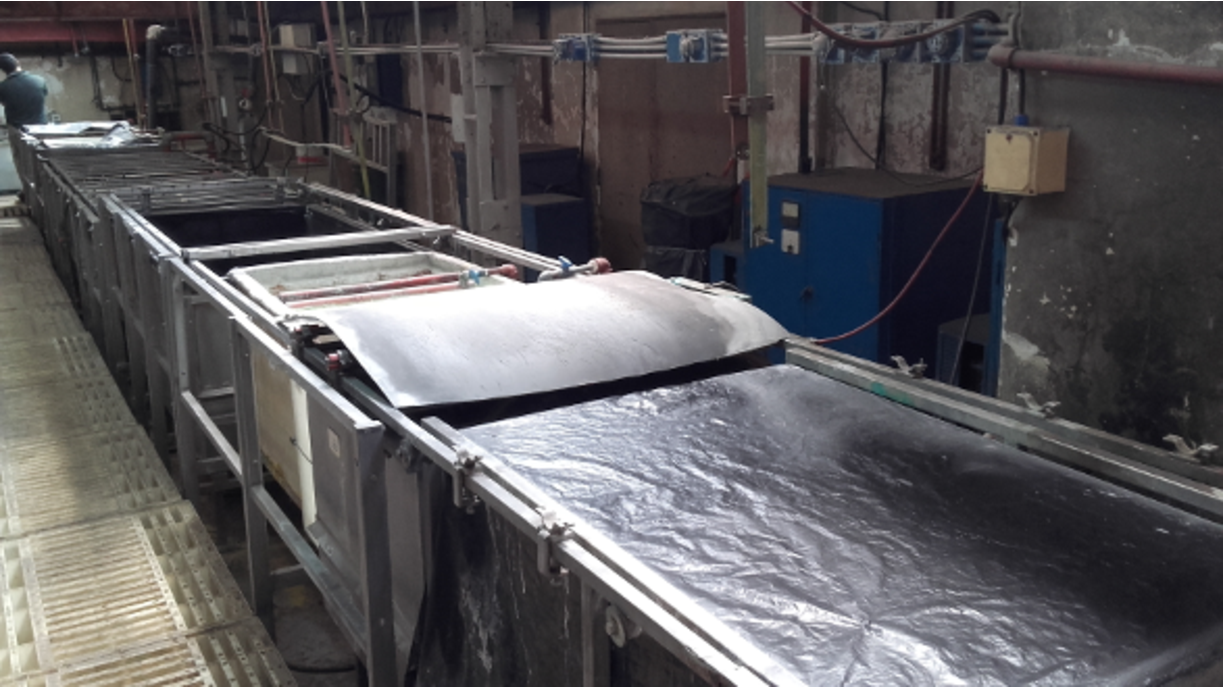
\includegraphics[width=.8\textwidth]{Figures/Cap_1/planta_actual}
	\caption{Linea de galvanizada actual operada manualmente.}
	\label{fig:planta_actual}
\end{figure}

En la Figura \ref{fig:planta_moderna} se puede ver como es una linea de producción totalmente automatizada del fabricante Eurocircuits de Bélgica \footnotemark.
\footnotetext{\url{https://www.eurocircuits.com}}

\begin{figure}[h]
	\centering
	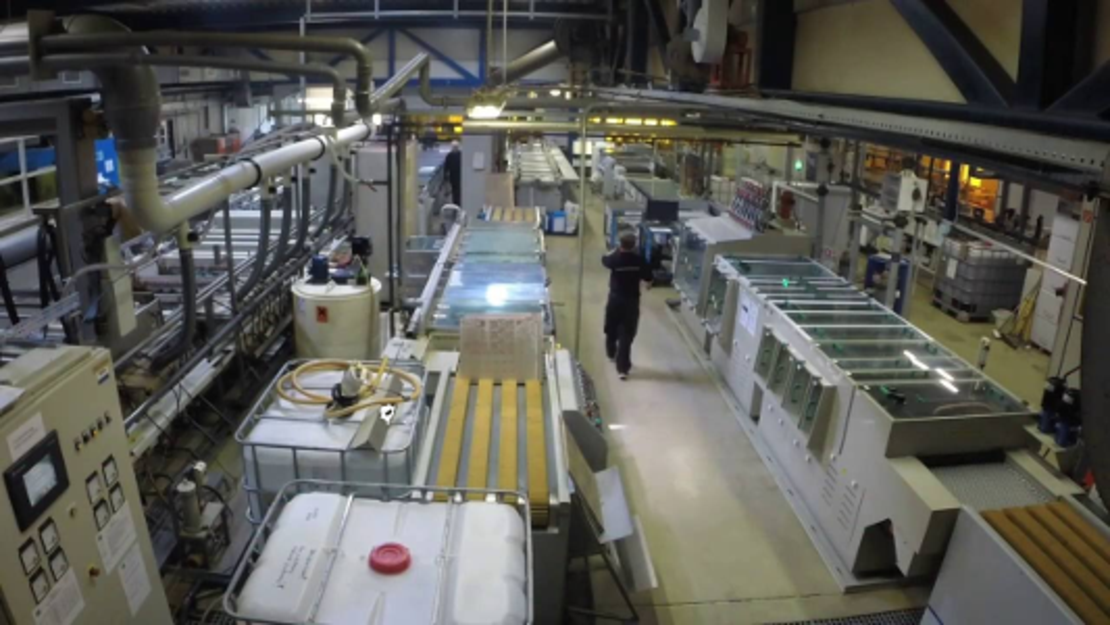
\includegraphics[width=.8\textwidth]{Figures/Cap_1/planta_moderna}
	\caption{ Ejemplo de una linea de galvanizada automatizada.}
	\label{fig:planta_moderna}
\end{figure}

\section{ Objetivo }

El objetivo fue diseñar un sistema de control sobre un hardware prototipo basado en un sistema embebido confiable y robusto, el cual funcionara como un modulo independiente de control y monitoreo por lo que tendría que ser fácilmente adaptable a los distintos configuraciones que podrían surgir en las distintas etapas de las linea de producción de los PCBs.
A su ves debería usarse un hardware adicional que implemente las interfaces necesarias para los distintos sistemas de control a utilizar en la futura planta y al mismo poder probarlo en un banco de prueba a cargo del fabricante.

\section{ Alcance }

Previo al desarrollo se limito el alcance del proyecto en los siguientes puntos:
\begin{itemize}
	\item Estudio preliminar de las arquitecturas adecuadas para la implementación del sistema principal y subsistemas.
	\item Diseño de alto nivel (arquitectura) del sistema.
	\item Diseño del sistema en lenguaje C.
	\item Plan de pruebas unitarias y ensayos (testbenchs) para cada subsistema.
	\item Plan de pruebas de integración y ensayos (testbenchs) para agrupaciones de subsistemas.
	\item Plan de pruebas del sistema y ensayos (testbenchs) para el sistema completo.
	\item Documentación del sistema y subsistemas que incluye:
	\begin{enumerate}
		\item Descripción de entradas y salidas (frecuencias, tamaño y tipos de datos, señales de control, etc.)
		\item Descripción de parámetros del sistema.
		\item Requerimientos funcionales implementados trazables a los requerimientos del proyecto (matriz de trazabilidad).
		\item Hipótesis de diseño, justificación de la elección del diseño, estudios previos y marco teórico.
		\item Diagrama de arquitectura.
		\item Reporte de ensayos realizados.
		\item Referencias bibliográficas.
	\end{enumerate}
	\item Análisis y construcción del banco de pruebas.
\end{itemize}
\hspace{1px}

Por otro lado se determino que el proyecto no incluiría el desarrollo de los siguientes puntos: 
\begin{itemize}
	\item Estudio de los sensores y actuadores, se basará dicha información en los datos dados por el cliente. 
	\item Análisis de mejor solución para implementación de sistema de reporte remoto de variables y registros históricos.
	\item Análisis y construcción del banco de prueba necesario.
	\item Test del sistema en lugar de producción. La planta se encontraba en reestructuración y modernización.
\end{itemize}



%----------------------------------------------------------------------------------------
%----------------------------------------------------------------------------------------





